\documentclass[11pt]{article}
\usepackage[a4paper,margin=0.9in]{geometry}
\usepackage{amsmath,amssymb,booktabs,graphicx,enumitem,xcolor,array}
\usepackage[hidelinks]{hyperref}
\usepackage{caption}
\setlength{\parindent}{0pt}\setlength{\parskip}{5pt}
\setlist{itemsep=2pt,topsep=3pt}
\renewcommand{\arraystretch}{1.2}
\newcommand{\T}{^{\top}}

\title{\textbf{Eigenfaces vs Fisherfaces: Project Report}}
\author{Shubh Karman Singh (26M0843) \quad Saumya Bajpai (26D0366)\\CS 740}
\date{24 November 2026}
\begin{document}
\maketitle

We reproduced Belhumeur, Hespanha and Kriegman, ``Eigenfaces vs.\ Fisherfaces'' (IEEE TPAMI 1997) in MATLAB, confirmed its main claim on Yale, found where it fails (ORL), and ran four experiments on choosing $m$, lighting angle, glasses and training-set size.

\section{Problem and algorithm}
The paper claims that Fisherfaces (PCA followed by LDA) recognise faces far more reliably than Eigenfaces (PCA) when lighting or expression changes, because LDA uses the labels to ignore variation within a person.
\begin{itemize}
\item \textbf{Eigenfaces:} subtract the mean face, keep the top $k$ eigenvectors of the total scatter $S_T$, project, classify by 1-nearest neighbour. PCA maximises $|W\T S_T W|$, so it keeps lighting variation too.
\item \textbf{Fisherfaces:} subtract the mean, reduce with PCA to $m$ dimensions (the paper uses $m=N-c$), solve $S_B w=\lambda S_W w$ and keep the top $c-1$ directions, then 1-NN. LDA maximises $|W\T S_B W|/|W\T S_W W|$.
\item \textbf{Why PCA first:} $\operatorname{rank} S_W\le N-c$, far below the number of pixels $d$, so $S_W$ is singular in pixel space.
\end{itemize}
\begin{center}
\begin{tabular}{lll}\toprule
 & ORL & Cropped Extended Yale B\\\midrule
Subjects & 40 & 38\\
Images per subject & 10 & 59--64\\
Image size (pixels) & $92\times112=10{,}304$ & $168\times192=32{,}256$\\
What varies & pose, expression, glasses & lighting only\\\bottomrule
\end{tabular}
\end{center}
The two databases are near-complements, so together they act as a controlled experiment.

\section{The mathematics}
Each image is flattened into a vector $x_i\in\mathbb R^d$. There are $N$ training images in $c$ classes; class $j$ has $n_j$ images and mean $\mu_j$, and $\mu$ is the overall mean.

\textbf{Scatter matrices.} Total spread, spread between class means, and spread within each class:
\[
S_T=\sum_{i=1}^{N}(x_i-\mu)(x_i-\mu)\T,\qquad
S_B=\sum_{j=1}^{c}n_j(\mu_j-\mu)(\mu_j-\mu)\T,\qquad
S_W=\sum_{j=1}^{c}\sum_{x_i\in X_j}(x_i-\mu_j)(x_i-\mu_j)\T .
\]
Writing $x_i-\mu=(x_i-\mu_j)+(\mu_j-\mu)$ and noting the cross terms sum to zero within each class gives
\[ S_T=S_B+S_W. \]

\textbf{Eigenfaces (PCA)} keep the directions of largest total spread; the columns of $W$ are the top $k$ eigenvectors of $S_T$:
\[ W_{pca}=\arg\max_{W\T W=I}\;|W\T S_TW|,\qquad S_Tv_l=\lambda_lv_l . \]
Since $d$ is huge, we use $L=X\T X$ ($N\times N$, $X$ = centred data): if $Lw=\mu w$ then $XX\T(Xw)=\mu(Xw)$, so $v=Xw/\|Xw\|$ is an eigenface.

\textbf{Fisherfaces (LDA)} maximise between-class spread relative to within-class spread:
\[ W_{fld}=\arg\max_W\;\frac{|W\T S_BW|}{|W\T S_WW|}. \]
For one direction $w$ the ratio is unchanged by scaling $w$, so fix the denominator and use a Lagrange multiplier:
\[ \max_w\; w\T S_Bw\ \ \text{s.t.}\ \ w\T S_Ww=1\;\Longrightarrow\; S_Bw=\lambda S_Ww,\qquad \lambda=\frac{w\T S_Bw}{w\T S_Ww}. \]
Each generalised eigenvalue is the Fisher score of its direction, so we keep the largest. With two classes this has the closed form $w\propto S_W^{-1}(\mu_1-\mu_2)$.

\textbf{Two rank bounds drive the whole method.}
\[ \operatorname{rank}S_B\le c-1,\qquad \operatorname{rank}S_W\le N-c\ll d. \]
$S_B$ has at most $c-1$ non-zero eigenvalues because $\sum_j n_j(\mu_j-\mu)=0$, so there are at most $c-1$ Fisherfaces. In each class the deviations $x_i-\mu_j$ sum to zero, so class $j$ adds only $n_j-1$ directions: $S_W$ is singular in pixel space. The paper therefore projects with PCA first:
\[ W_{opt}=W_{pca}W_{fld},\qquad W_{pca}\in\mathbb R^{d\times m},\ \ W_{fld}\in\mathbb R^{m\times(c-1)},\ \ m=N-c. \]

\textbf{Solving $S_Bw=\lambda S_Ww$.} We factor the reduced $S_W=R\T R$ (Cholesky) and substitute $z=Rw$, which turns it into a symmetric eigenproblem; Fisherfaces come out $S_W$-orthogonal, not orthogonal:
\[ \left(R^{-\top}S_BR^{-1}\right)z=\lambda z,\qquad w=R^{-1}z,\qquad w_i\T S_Ww_j=0\ (i\ne j). \]

\section{Implementation and verification}
Everything is one MATLAB script (\texttt{fisherfaces\_project.m}): PCA through the small matrix $L=X\T X$, LDA solved by Cholesky whitening of $S_W$, and 1-NN in squared Euclidean distance with test images centred on the training mean. Before trusting any accuracy, we checked the implementation against the theory.

\subsection*{Eigenfaces: steps}
\begin{enumerate}
\item Load each image, convert to double, flatten with \texttt{im(:)}; training images form the columns of a $d\times N$ matrix.
\item Compute the mean face $\bar x$ and centre: $X=[x_1-\bar x,\dots,x_N-\bar x]$.
\item Form $L=X\T X$ ($N\times N$), take its eigenvectors with \texttt{eig} and sort eigenvalues in descending order.
\item Map back and normalise: $V=XW$, each column divided by its norm. Drop the last one (eigenvalue 0, since $\operatorname{rank}X\le N-1$).
\item Keep the top $k$ columns, $V_k$; training features are $\alpha=V_k\T X$.
\item Test image $z$: features $V_k\T(z-\bar x)$ with the training mean, then 1-nearest neighbour in squared Euclidean distance.
\end{enumerate}

\subsection*{Fisherfaces: steps}
\begin{enumerate}
\item Centre exactly as above.
\item PCA to $m$ dimensions (paper: $m=N-c$): $W_{pca}$ = first $m$ eigenfaces, reduced data $Z=W_{pca}\T X$ ($m\times N$). Its overall mean is zero because $X$ is centred.
\item In this $m$-dimensional space, loop over classes: class mean $\bar z_j$, then $S_B \mathrel{+}= n_j\bar z_j\bar z_j\T$ and $S_W\mathrel{+}=(z_i-\bar z_j)(z_i-\bar z_j)\T$. Both are $m\times m$, never $d\times d$.
\item Check $\operatorname{rank}S_W=m$ and that its condition number is finite.
\item Solve $S_Bw=\lambda S_Ww$ by Cholesky whitening, sort $\lambda$ descending, keep the top $c-1$ eigenvectors: $W_{fld}$ ($m\times(c-1)$).
\item Combine $W_{opt}=W_{pca}W_{fld}$ ($d\times(c-1)$); each column reshaped to an image is a Fisherface.
\item Project training and test images with $W_{opt}$ (test centred on the training mean) and classify by 1-nearest neighbour.
\end{enumerate}
\begin{center}
\begin{tabular}{lll}\toprule
Matrix & Size & ORL-32 ($N=192$, $c=32$)\\\midrule
$X$ (centred images) & $d\times N$ & $10{,}304\times192$\\
$L=X\T X$ & $N\times N$ & $192\times192$\\
$W_{pca}$ & $d\times(N-c)$ & $10{,}304\times160$\\
$S_B$, $S_W$ (reduced) & $(N-c)\times(N-c)$ & $160\times160$\\
$W_{opt}$ (Fisherfaces) & $d\times(c-1)$ & $10{,}304\times31$\\\bottomrule
\end{tabular}
\end{center}

\subsection*{Verification checks}
\begin{center}
\begin{tabular}{lll}\toprule
Check & Theory & Measured\\\midrule
$S_T=S_B+S_W$ & exact & $\le 8.6\times10^{-16}$ relative\\
$\operatorname{rank}S_W\le N-c$ (Yale) & $\le1482$ & 1482\\
$\operatorname{rank}S_B=c-1$ (ORL-32) & 31 & 31\\
Eigenfaces orthonormal & $V\T V=I$ & $9.1\times10^{-14}$\\
Fisherfaces $S_W$-orthogonal, not orth. & $w_i\T S_Ww_j=0$ & $3.8\times10^{-13}$ vs 0.499\\
Our solver vs \texttt{eig(Sb,Sw,'chol')} & same & $\le7.8\times10^{-16}$ relative\\
Toy data: closed-form $w$ maximises $J(w)$ & maximum & beats a 6,283-direction grid\\\bottomrule
\end{tabular}
\end{center}
We also reproduced the HW3 Eigenfaces numbers exactly. Two protocol issues surfaced only through these checks: a duplicated Yale file appeared as a one-unit rank deficiency in $S_W$, and the text-sorted Yale split turned out to be biased (Experiment 2).

\section{Main result}
The paper's claim holds on Yale and fails on ORL: Fisherfaces cut Yale error from 30.0\% to 2.9\% (random split), but lose to Eigenfaces on ORL.
\begin{center}\small
\begin{tabular}{lccccc}\toprule
Recognition rate (\%) & Correlation & Eigen (best $k$) & Eigen ($k=c-1$) & Eigen w/o top 3 & Fisherfaces\\\midrule
Yale-38, random split & 85.2 & 70.0 & 50.2 & 89.0 & \textbf{97.1}\\
Yale-38, HW3 split & 43.0 & 34.2 & 29.5 & 58.7 & \textbf{67.2}\\
ORL-32 & 91.4 & \textbf{95.3} & 94.5 & 87.5 & 90.6\\
ORL-40 & 91.2 & \textbf{93.8} & 94.4 & 86.9 & 84.4\\\bottomrule
\end{tabular}
\end{center}
Fisherfaces always use exactly $c-1$ features, so the $k=c-1$ column is the fair comparison. On Yale, Fisherfaces also beat dropping the top three eigenfaces (97.1 vs 89.0): that trick assumes the nuisance is exactly 3-dimensional, while LDA learns it from the labels.

\section{Experiments}
\subsection{Choosing the PCA dimension $m$ before LDA}
The paper's $m=N-c$ is not the best choice on either database. On ORL-32, $m=60$ gives 95.3\% (tying the best Eigenfaces) against 90.6\% at $m=N-c=160$; on Yale, $m=1000$ gives 97.0\% against 95.7\% at $m=1482$.

The condition number of the projected $S_W$ explains it: over ORL's last 20 dimensions it jumps from $5.8\times10^3$ to $7.9\times10^7$ (Yale: $2.6\times10^6$ to $2.2\times10^{11}$). Those last directions are estimated from almost no data, and LDA inverts $S_W$, so they receive the largest weight. Rates were measured on the held-out test images.
\begin{center}
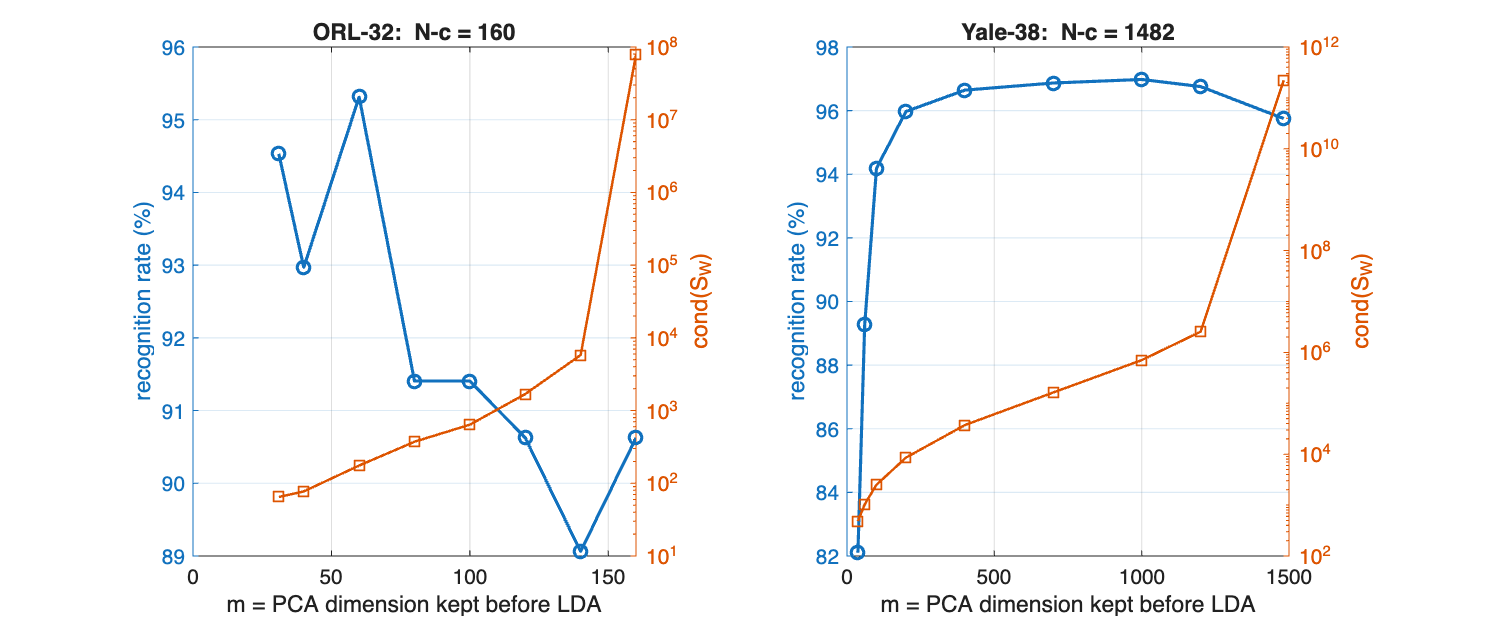
\includegraphics[width=0.85\textwidth]{fig-002.png}
\captionof{figure}{Recognition rate (left axis) and condition number of $S_W$ (right axis, log scale) against $m$, for ORL-32 and Yale-38.}
\end{center}

\subsection{Illumination angle}
Unseen lighting angles roughly halve every method's accuracy, and Fisherfaces degrade least. Sorting Yale filenames as text puts every positive-azimuth image (A+) before every negative one (A$-$), so the HW3 ``first 40'' split trains on $+$azimuth lamps and tests on $-20^\circ$ to $-130^\circ$. We compared it with a random split of the same size.
\begin{center}
\begin{tabular}{lcc}\toprule
Recognition rate (\%) & Unseen angles (HW3 split) & Random split\\\midrule
Correlation & 43.0 & 85.2\\
Eigenfaces (best $k$) & 34.2 & 70.0\\
Eigenfaces w/o top 3 & 58.7 & 89.0\\
Fisherfaces & 67.2 & 97.1\\\bottomrule
\end{tabular}
\end{center}
The ranking of methods is the same under both splits. Fisherfaces' advantage over Eigenfaces is larger on unseen angles ($1.96\times$) than on the random split ($1.39\times$).

Per-subset results (train on lamps within $12^\circ$ of the camera axis, test at $\le25^\circ$, $\le50^\circ$, $\le77^\circ$ and $>77^\circ$): [fill in, or delete this line].

\subsection{Glasses vs no glasses}
Relabelling ORL images as glasses / no glasses gives two classes, so LDA produces a single Fisherface, $w\propto S_W^{-1}(\mu_1-\mu_2)$. PCA's subspace depends only on $S_T$, which does not change with the labels.
\begin{center}
\begin{tabular}{lcc}\toprule
Error (\%) & Ours & Paper (Yale)\\\midrule
Eigenfaces & [\_\_] & 52.6\\
Fisherfaces & [\_\_] & 5.3\\\bottomrule
\end{tabular}
\end{center}
[Add: number of glasses / no-glasses images, the evaluation protocol, and one line on what the single Fisherface highlights.]

\subsection{Training images per class}
On Yale, Fisherfaces beat Eigenfaces at every training-set size, even with two images per person (43.0\% vs 19.9\%), when $S_W$ gets only one degree of freedom per class. The advantage shrinks as data grows, from $2.16\times$ at 2 images to $1.40\times$ at 40 (94.2\% vs 67.3\%). Because lighting dominates, even a poorly estimated $S_W$ points roughly the right way. With one image per person Fisherfaces cannot be computed, since $S_W=0$.
\begin{center}
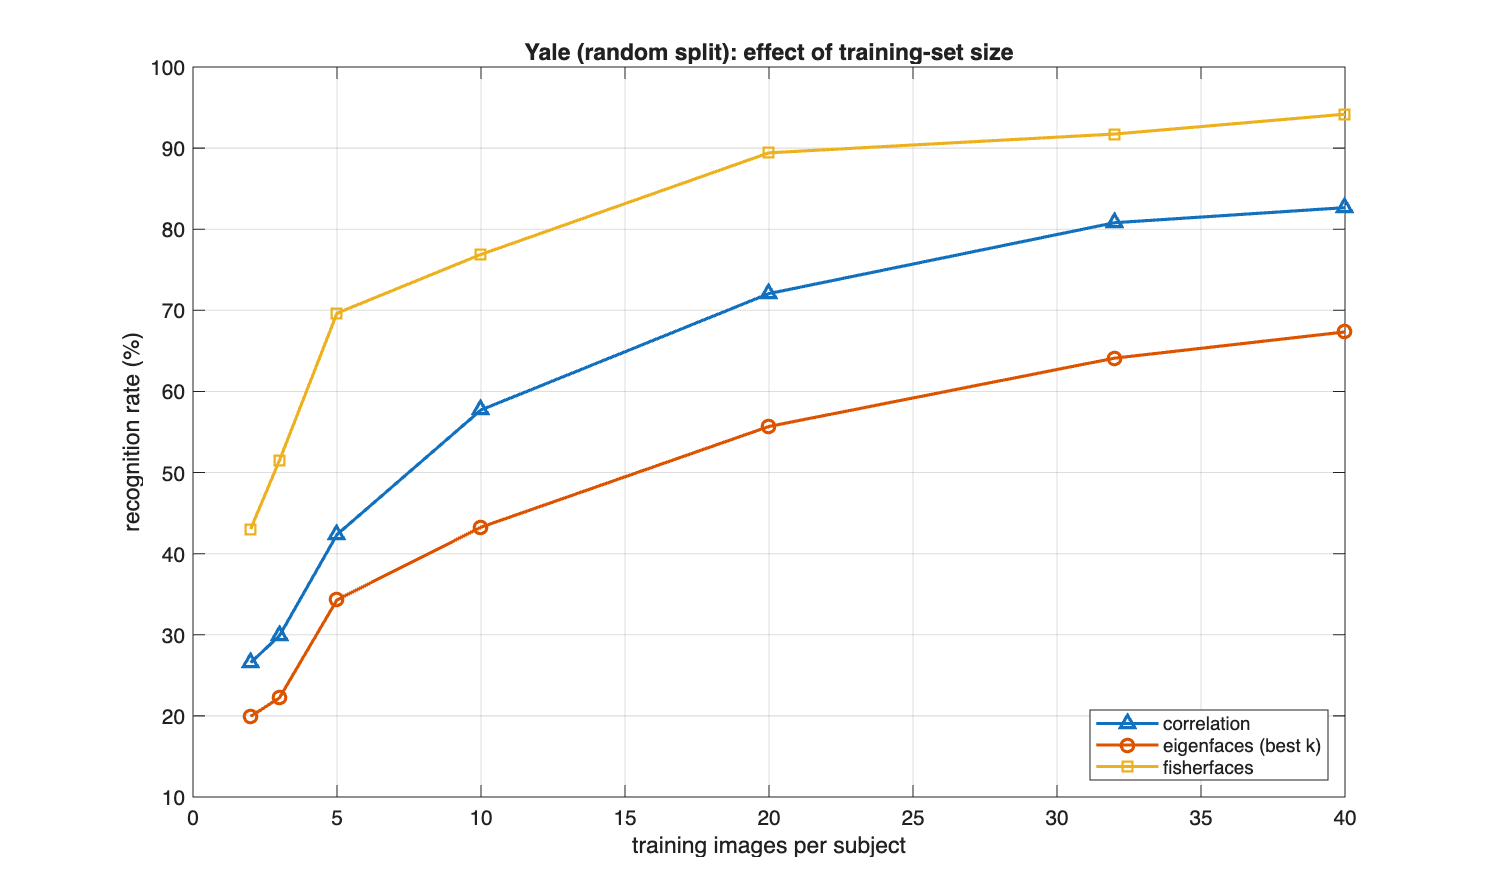
\includegraphics[width=0.62\textwidth]{fig-003.png}
\captionof{figure}{Yale, random split: recognition rate against training images per subject.}
\end{center}

\section{Observations}
\textbf{Fisherfaces lose on ORL because $S_W$ is estimated from too little data.} With 6 images per person, each class contributes 5 independent deviations, so ORL-32 gives 160 degrees of freedom to estimate a $160\times160$ matrix (about 12,800 entries); Yale gives 39 per person. Adding classes makes it worse: from 32 to 40 people, Fisherfaces fall from 90.6\% to 84.4\% while Eigenfaces barely move (95.3\% to 93.8\%). A smaller $m$ (Experiment 1) recovers the gap.

\textbf{Fisherfaces look like noise, and the whitening step predicts it.} Eigenfaces are smooth and face-like; Fisherfaces are speckled. LDA scales each eigen-direction of $S_W$ by $1/\sqrt\lambda$, and small-$\lambda$ directions (fine detail a person keeps) are high-frequency. Measured on ORL-32, Fisherfaces have a $3.85\times$ higher frequency centroid (0.118 vs 0.031) and $11\times$ the share of high-frequency power (25.9\% vs 2.3\%).
\begin{center}
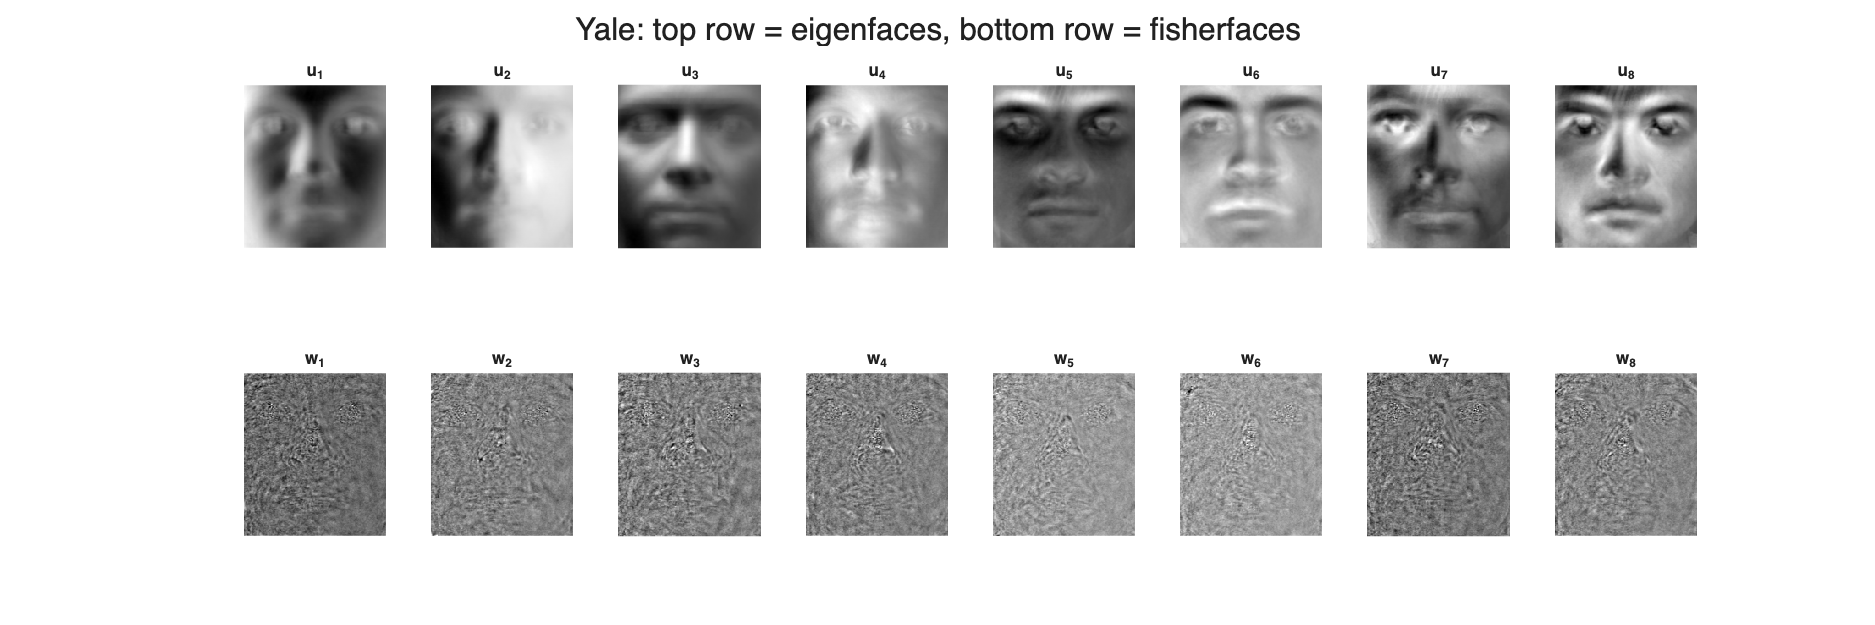
\includegraphics[width=0.9\textwidth]{fig-004.png}
\captionof{figure}{Yale: first eight eigenfaces (top row) and first eight Fisherfaces (bottom row).}
\end{center}

\section{Conclusions}
\begin{enumerate}
\item The paper's claim holds where the within-person nuisance is large and structured: under lighting change, Fisherfaces cut Yale error from 30.0\% to 2.9\%.
\item It is a claim about nuisance structure and data, not ``LDA is always better'': on ORL (pose and expression, 6 images per person) Eigenfaces win.
\item $m=N-c$ is the weakest part of the recipe: it is the worst-conditioned valid choice, and a smaller $m$ does better on both databases (95.3\% vs 90.6\% on ORL, 97.0\% vs 95.7\% on Yale).
\item Supervision helps most when conditions are hard: Fisherfaces extrapolate better to unseen lighting ($1.96\times$ vs $1.39\times$) and still win on Yale with two images per person.
\item Protocol mattered as much as the algorithm: the text-sorted Yale split roughly halved every method's score, and was found by checking numbers against theory.
\end{enumerate}
\end{document}
